
\chapter{Testowanie}
\section{Frontend}
Testy w części frondendowej aplikacji wykonywane są przy pomocy platformy programistycznej Jest. W projekcie można wyróżnić podział na dwa typy testów. Pierwszym typem są testy spójności magazynu Vuex. Przykładowym testem tego typu jest test przypisanie tokenu JWT~(zob.~listing~\ref{lst:vuextest}). Celem testu jest sprawdzenie, czy funkcje odpowiadające za zapisywanie i odczytywanie danych zostały poprawnie zdefiniowane.
\begin{lstlisting}[caption=Test spójności magazynu Vuex,label={lst:vuextest}] 
describe('mutations', () => {
  test('setToken', () => {
    const token = "exampletoken"
    const state = {
      token: ""
    }
    store.commit('SET_TOKEN', { token })
    expect(store.getters.getToken.token).toBe(token)
  })
\end{lstlisting}

Drugim typem testów są testy interfejsu użytkownika. Przykładem takiego testu jest test przycisku, który odpowiada za zwiększanie liczby prowadzonych przez nauczyciela przedmiotów~(zob.~listing~\ref{lst:uitest}). Celem testu jest sprawdzenie, czy akcja wykonana przez użytkownika, w tym przypadku symulowana, skutkuje odpowiednią zmianą zmiennych w kodzie aplikacji. 
\begin{lstlisting}[caption=Test interfejsu użytkownika,label={lst:uitest}] 
describe('userInput', () => {
  test('addSubject', async () => {
    const wrapper = mount(Step2)
    const button = wrapper.find('addSubjectButton')

    expect(subjectNumber).toBe(0)
    await button.trigger('click')
    expect(subjectNumber).toBe(1)
})})
\end{lstlisting}
\section{Backend}
\subsection{Testowanie manualne}

Część backendowa, testowana była w dużym stopniu manualnie. Głównym narzędziemy była aplikacja Postman. Przykładowe zapytanie wraz z odpowiedzią na rysunku ~\ref{rys:postman}

\begin{figure}[H]
	\centering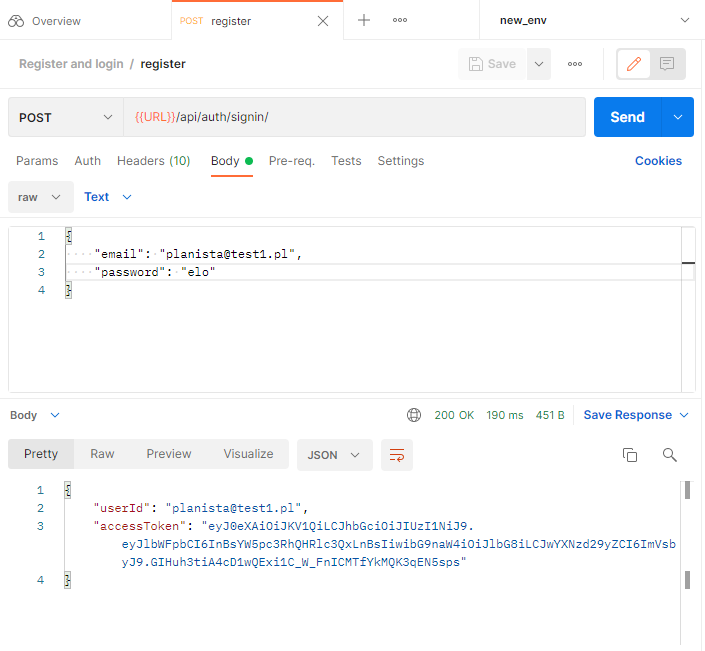
\includegraphics[width=\textwidth]{figures/postman}
	\caption{Przykładowe zapytanie oraz odpowiedź w Postman}\label{rys:postman}
\end{figure}

Na zaawansowanych etapach implementacji, testy wykonywane były również z pomocą aplikacji frontendowej, dzięki czemu można była na bieżąco weryfikować integrację.

\subsection{Testy automatyczne}
Testami automatycznymi objęte zostały widoki oraz adresy URL. Do testowania widoków, wykorzystywane są testy integracyjne, natomiast do adresów testy jednostkowe. W obu przypadkach wykorzystywane są gotowe rozwiązania zaimplementowane w Django. Testy jednostkowe, sprawdzające poprawność implementacji adresów internetowych, sprawdzają czy podczas wysłania zapytania na dany adres, wywoływana jest opowiednia funkcja. Przykład implementacji takiego testu na listingu ~\ref{lst:TestJednostkowy}

\begin{lstlisting}[language=Python, caption=Implementacja przykładowego testu jednostkowego, label={lst:TestJednostkowy}]
	class TestUrls(SimpleTestCase):
	
		def test_add_user(self):
			url = reverse('user')
			self.assertEquals(resolve(url).func, add_user)
\end{lstlisting}

Natomiast testy integracyjne, odpowiadające za widoki, mają za zadanie sprawdzić czy widok zwrócił odpowiednią odpowiedź HTPP. Przykład takiego testu na listingu ~\ref{lst:TestIntegracyjny}

\begin{lstlisting}[language=Python, caption=Implementacja przykładowego testu integracyjnego, label={lst:TestJednostkowy}]
	class TestViews(TestCase):
	
		def test_add_user_POST(self):
	
			email = 'test1@test2@.com'
			client = Client()
			url = reverse('user')
			
			Planners.objects.create(
			planneremail = email,
			login = 'test',
			password = 'test'
			)
			
			response = client.post(url, {
				'Sukces': 'Pomyslnie dodano uzytkownika'
			})
			
			self.assertEquals(response.status_code, 200)
\end{lstlisting}


\section{Algorytm}

